%
% $RCSfile: enumerative_scheme.tex,v $
%
% Copyright (C) 2002-2008. Christian Heller.
%
% Permission is granted to copy, distribute and/or modify this document
% under the terms of the GNU Free Documentation License, Version 1.1 or
% any later version published by the Free Software Foundation; with no
% Invariant Sections, with no Front-Cover Texts and with no Back-Cover
% Texts. A copy of the license is included in the section entitled
% "GNU Free Documentation License".
%
% http://www.cybop.net
% - Cybernetics Oriented Programming -
%
% http://www.resmedicinae.org
% - Information in Medicine -
%
% Version: $Revision: 1.1 $ $Date: 2008-08-19 20:41:06 $ $Author: christian $
% Authors: Christian Heller <christian.heller@tuxtax.de>
%

\subsubsection{Enumerative Scheme}
\label{enumerative_scheme_heading}
\index{Enumerative Scheme}
\index{Enumerative Coding Scheme}
\index{Taxonomic Classification}
\index{International Classification of Diseases}
\index{ICD}

An \emph{Enumerative Coding Scheme} lists, within the scheme, \emph{all} phrases
ever to be used, and gives each of them its own code for reference. The phrases
can be very long and detailed. The list of phrases provided is \emph{finite},
and it is \emph{fixed}.

\begin{table}[ht]
    \begin{center}
        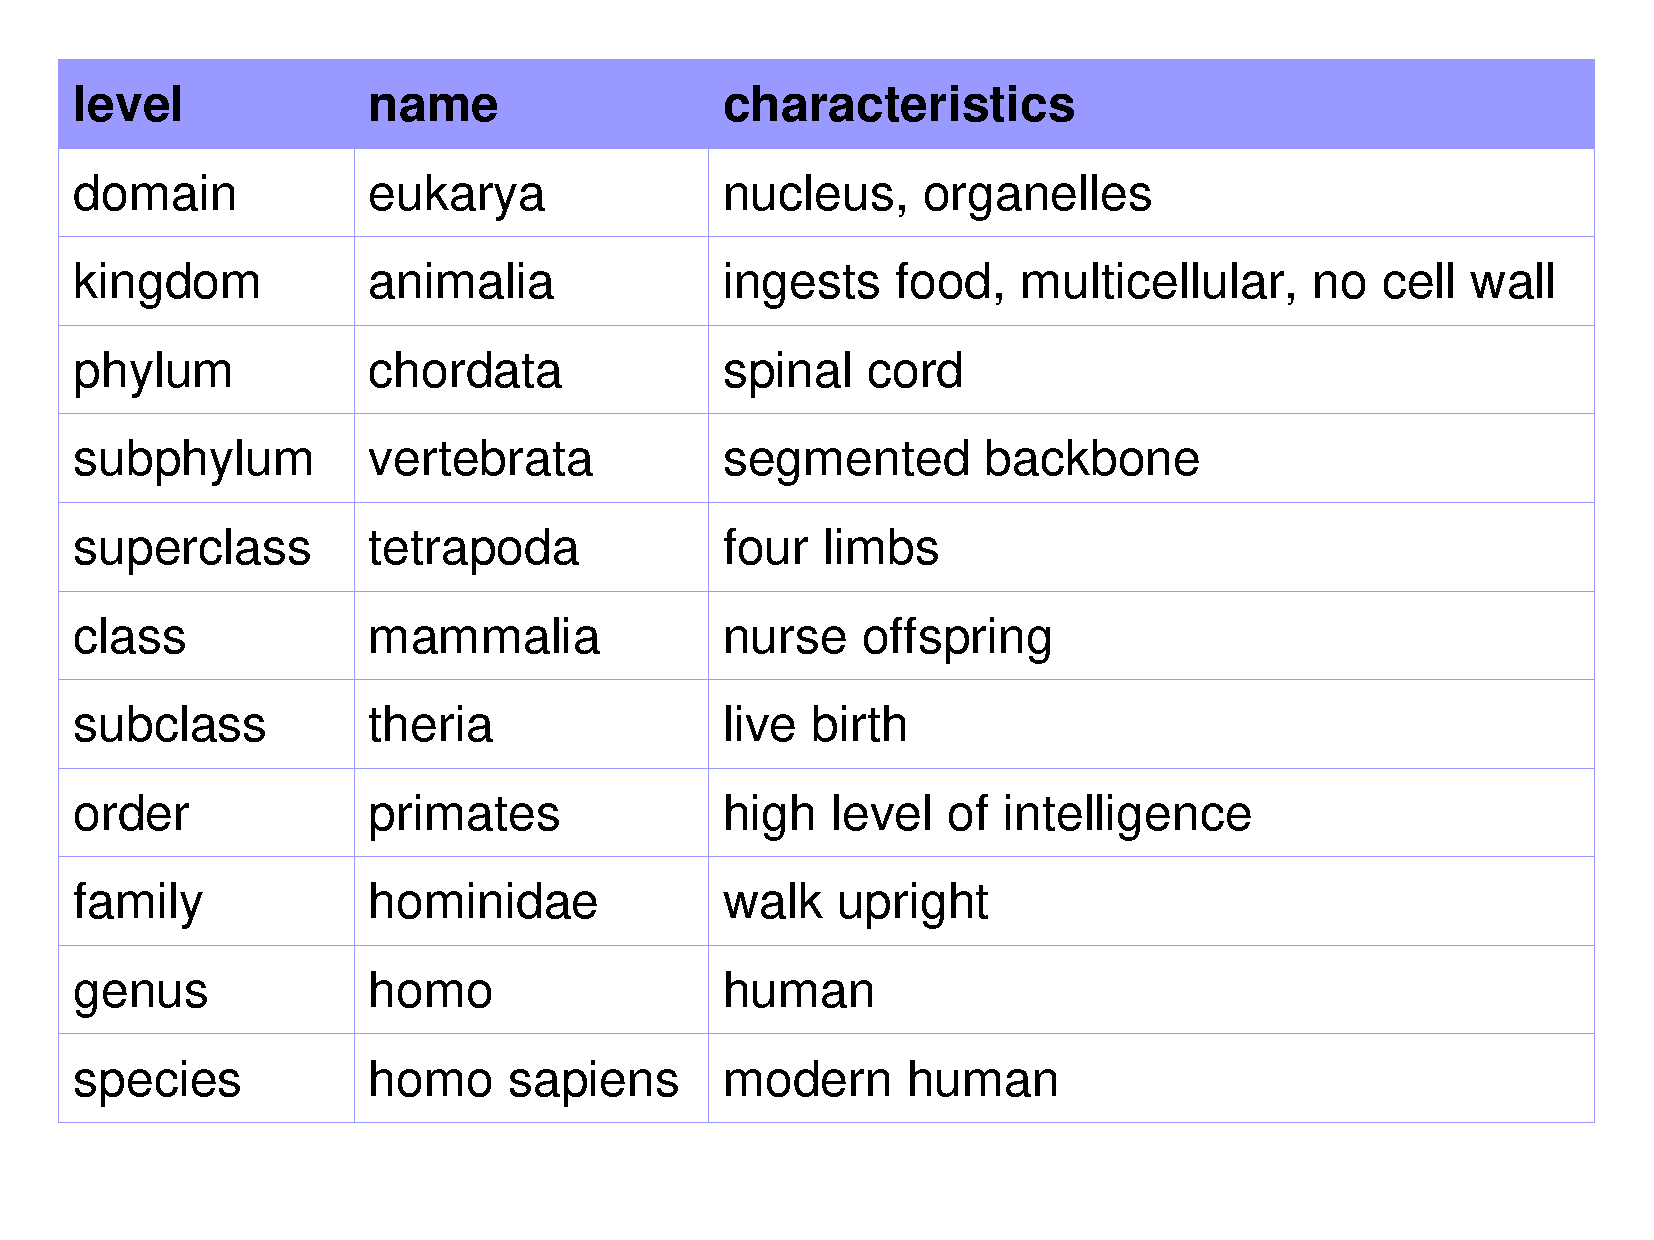
\includegraphics[scale=0.4,angle=-90]{graphic/taxonomy.pdf}
        \caption{Taxonomic Classification of the Animal Kingdom}
        \label{taxonomy_table}
    \end{center}
\end{table}

A very familiar example of an enumerated scheme is the traditional taxonomic
classification of the animal kingdom (figure \ref{taxonomy_table}). Most of the
existing medical terminologies, listing names of diseases, of surgical
operations and the like, are also enumerative. One example is the
\emph{International Classification of Diseases} (ICD) (chapter
\ref{res_medicinae_heading}).

After \cite{rogers}, attempting to enumerate in advance all useful phrases
inevitably encounters two serious problems concerning the \emph{Scale} and
\emph{Organisation}. Terminologies become:

\begin{enumerate}
    \item \emph{Scale:} too big to maintain, which results in inconsistent data
        that cannot be analysed anymore
    \item \emph{Organisation:} pre-categorised, which does not allow terms to
        be simultaneously placed under all different categories that are valid
\end{enumerate}

A further limitation is caused by unfavourable technical choices. The code often
serves two purposes. It is: the unique identifier of a concept and the means of
representing the relative organisation of a concept. So the common practice of
restricting the physical length of a code also restricts the levels of
organisation.
